\documentclass[12pt letter]{report}
\input{../template/preamble}
\input{../template/macros}
\input{../template/letterfonts}

\usepackage{parskip}
\usepackage{tikz}
\usetikzlibrary{matrix, positioning, arrows, decorations.pathreplacing, calc}
\usepackage{colortbl}
\usepackage{xcolor}
\title{\Huge{Homework 3}}
\author{\huge{Madiba Hudson-Quansah}}
\date{}


\begin{document}
\maketitle
\newpage

\qs{}{
  Describe the effect that a single stuck-at-0 fault (i.e., the signal is always 0 regardless of what it should be) would have for the signals shown below in the single-cycle Datapath. Which instructions, if any, will not work correctly? Explain why.
  Consider each of the following faults separately:
  \begin{enumerate}
    \item  RegWrite = 0
    \item  RegDst = 0
    \item  ALUScr = 0
    \item  MemtoReg = 0
    \item  Branch = 0
  \end{enumerate}
}

\sol{
  \begin{enumerate}
    \item In the case of  RegWrite stuck at 0 it would prevent the register file from writing to the registers. This means that any instruction that
          requires writing to a register, i.e. ALU, Load and Store instructions will not work correctly.
    \item In the case of a RegDst stuck at 0 it would cause in the destination register to always come from the rt field of the instruction even if
          the instruction is not an I-type instruction. This means that R-type instructions which specify the destination register in the rd field will not work correctly, inputting the result into the wrong register.
    \item In the case of ALUSrc stuck at 0 it would mean the ALU operands would always from a register. This would affect all instructions that depend on the ALU, i.e. all R-type instructions, Load/Store instructions and even branch instructions as they depend on the ALU to calculate the branch address.
    \item In the case of  MemtoReg stuck at 0 it would prevent data in memory from being written to the register file correctly. This means that any instruction
          that requires writing to the register file from memory, i.e. Load instructions, will not work correctly.
    \item In the case of Branch stuck at 0 it would prevent conditional branching entirely.
  \end{enumerate}
}

\qs{}{
  Repeat question 1 but this time consider stuck-at-1 faults (the signal is always 1).
}

\sol{
  \begin{enumerate}
    \item In the case of RegWrite stuck at 1 it would prevent the register file from writing to the registers correctly. This means that any instruction that
          requires writing to a register, i.e. ALU, Load and Store instructions will not work correctly and would always write to the register file potentially leading to nonsensical data being written to the register file.
    \item In the case of RegDst stuck at 1 it would cause the destination register to always come from the rd field of the instruction even if the instruction is not a R-type instruction. This means in the case of an I-type instruction, the destination register would be determined by the first 5 bits of the immediate field leading to incorrect registers being written to and possible out of bounds errors.
    \item In the case of ALUScr stuck at 1 it would mean the ALU operands would always from from an immediate value even if the instruction is not an immediate type instruction. This would affect all instructions that depend on the ALU, i.e. all R-type instructions, Load/Store instructions and even branch instructions as they depend on the ALU to calculate the branch address.
    \item In the case of a MemtoReg stuck at 1 it would always write data from memory to the register file in all situations. This could potentially
          lead to nonsensical data being written to the register file as the data being written to the register file may not be the correct data and would affect Load instructions.
    \item In the case of Branch stuck at 1 it would cause the CPU to interpret all instructions as conditional branch instructions causing non-deterministic behaviour. This would affect all instructions.
  \end{enumerate}
}

\qs{}{
  We wish to add the instruction jalr (jump and link register) to the single-cycle Datapath. Add any necessary datapath and control signals and draw the result datapath. Show the values of the control signals to control the execution of the jalr instruction.
  The jump and link register instruction is described below:
}

\sol{

}

\qs{}{
  Suppose we add the multiply and divide instructions. The operation times are as follows:
  Instruction memory access time = 190 ps,      Data memory access time = 190 ps,
  Register file read access time = 150 ps, 	Register file write access = 150 ps
  ALU delay for basic instructions = 190 ps,      ALU delay for multiply or divide = 550 ps
  Ignore the other delays in the multiplexers, control unit, sign-extension, etc.
  Assume the following instruction mix: 30\% ALU, 15\% multiply \& divide, 20\% load, 10\% store, 15\% branch, and 10\% jump.
  \begin{enumerate}
    \item What is the total delay for each instruction class and the clock cycle for the single-cycle CPU design?
    \item Assume we fix the clock cycle to 200 ps for a multi-cycle CPU, what is the CPI for each instruction class and the speedup over a fixed-length clock cycle?
  \end{enumerate}
}
\sol{
  \begin{enumerate}
    \item
          ALU - IF (Ins access), ID (ignored), EX (Reg read, ALU basic), WB (Reg write), i.e. $190 + 150+ 190 + 150 = 680$ \\
          MUL/DIV - IF (Ins access), ID(ignored), EX(Reg read, ALU mul/div), WB (Reg write), i.e. $190 + 150+ 550 + 150 = 1040$ \\
          Load - IF (Ins access), ID (ignored), EX(Reg read, ALU basic), MEM (Data access), WE (Reg write), i.e. $190 + 150 + 190 + 190 + 150 = 870$ \\
          Store - IF (Ins access), ID (ignored), EX(Reg read, ALU basic), MEM (Data access), i.e. $190 + 150 + 190 + 190 = 720$ \\
          Branch - IF (Ins access), ID (ignored), EX(Reg read, ALU basic), i.e. $190 + 150 + 190 = 530$ \\
          Jump - IF (Ins access), ID (ignored), i.e. $190$ \\
          Clock cycle = $1040 \text{ps}$ \\
    \item
          ALU - 4 cycles
          MUL/DIV - 6 cycles
          Load - 5 cycles
          Store - 5 cycles
          Branch - 3 cycles
          Jump - 1 cycle
          \begin{align*}
            \text{CPI} & = 4 \times 0.3 + 6 \times 0.15 + 5 \times 0.2 + 5 \times 0.1 + 3 \times 0.15 + 0.1 \\
                       & = 4.05
          \end{align*}
          Speedup:
          \begin{align*}
            \text{Multi-Clock cycle} & = 200 \times 4.05  \\
                                     & = 810              \\
            \\
            \text{Speedup}           & = \frac{1040}{810} \\
                                     & \approx 1.3        \\
          \end{align*}

  \end{enumerate}
}

\qs{}{
  Identify all the RAW data dependencies in the following code. Which dependencies are data hazards that will be resolved by forwarding? Which dependencies are data hazards that will cause a stall? Using a graphical representation of the pipeline, show the forwarding paths and stalled cycles if any.
}

\sol{
  \begin{itemize}
    \item Instruction 2 depends on instruction $\$3$ which is written by instruction 1. This can  be solved by forwarding the result of instruction 1 to instruction 2.
    \item Instruction 3 depends on $\$3$ which is written by instruction 1. This can be solved by forwarding the result of instruction 1 to instruction 3.
    \item Instruction 4 depends on $\$3$ which is written by instruction 1. This can be solved by forwarding the result of instruction 1 to instruction 4.
    \item Instruction 4 depends on $\$6$, which is written by instruction 3. This will cause a stall as value of $\$6$ is only available after  the MEM stage of instruction 3.
  \end{itemize}

  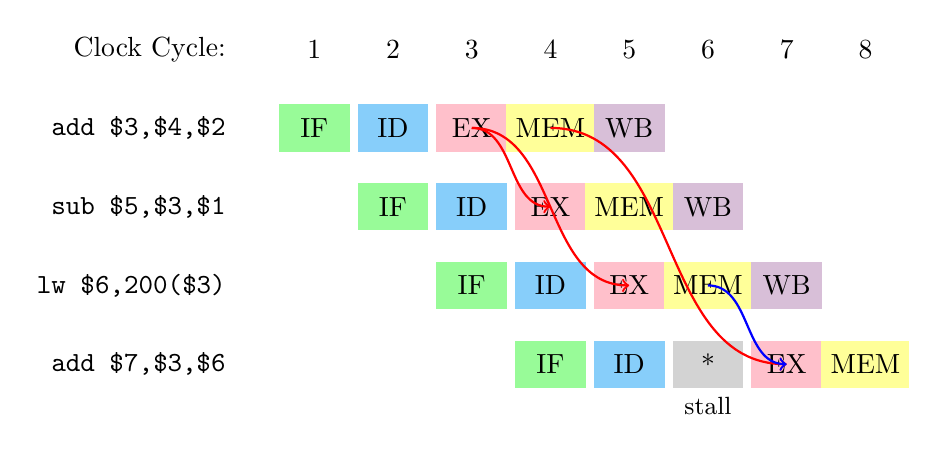
\begin{tikzpicture}
    % Define colors
    \definecolor{ifcolor}{RGB}{152, 251, 152}
    \definecolor{idcolor}{RGB}{135, 206, 250}
    \definecolor{excolor}{RGB}{255, 192, 203}
    \definecolor{memcolor}{RGB}{255, 255, 153}
    \definecolor{wbcolor}{RGB}{216, 191, 216}
    \definecolor{stallcolor}{RGB}{211, 211, 211}

    % Stage labels
    \node[anchor=east] at (0,0) {Clock Cycle:};
    \foreach \x in {1,...,8}
    \node[anchor=center] at (\x,0) {\x};

    % Instruction labels
    \node[anchor=east] at (0,-1) {\texttt{add \$3,\$4,\$2}};
    \node[anchor=east] at (0,-2) {\texttt{sub \$5,\$3,\$1}};
    \node[anchor=east] at (0,-3) {\texttt{lw \$6,200(\$3)}};
    \node[anchor=east] at (0,-4) {\texttt{add \$7,\$3,\$6}};

    % Pipeline stages for add $3,$4,$2
    \node[fill=ifcolor, minimum width=0.9cm, minimum height=0.6cm] at (1,-1) {IF};
    \node[fill=idcolor, minimum width=0.9cm, minimum height=0.6cm] at (2,-1) {ID};
    \node[fill=excolor, minimum width=0.9cm, minimum height=0.6cm] at (3,-1) {EX};
    \node[fill=memcolor, minimum width=0.9cm, minimum height=0.6cm] at (4,-1) {MEM};
    \node[fill=wbcolor, minimum width=0.9cm, minimum height=0.6cm] at (5,-1) {WB};

    % Pipeline stages for sub $5,$3,$1
    \node[fill=ifcolor, minimum width=0.9cm, minimum height=0.6cm] at (2,-2) {IF};
    \node[fill=idcolor, minimum width=0.9cm, minimum height=0.6cm] at (3,-2) {ID};
    \node[fill=excolor, minimum width=0.9cm, minimum height=0.6cm] at (4,-2) {EX};
    \node[fill=memcolor, minimum width=0.9cm, minimum height=0.6cm] at (5,-2) {MEM};
    \node[fill=wbcolor, minimum width=0.9cm, minimum height=0.6cm] at (6,-2) {WB};

    % Pipeline stages for lw $6,200($3)
    \node[fill=ifcolor, minimum width=0.9cm, minimum height=0.6cm] at (3,-3) {IF};
    \node[fill=idcolor, minimum width=0.9cm, minimum height=0.6cm] at (4,-3) {ID};
    \node[fill=excolor, minimum width=0.9cm, minimum height=0.6cm] at (5,-3) {EX};
    \node[fill=memcolor, minimum width=0.9cm, minimum height=0.6cm] at (6,-3) {MEM};
    \node[fill=wbcolor, minimum width=0.9cm, minimum height=0.6cm] at (7,-3) {WB};

    % Pipeline stages for add $7,$3,$6 with stall
    \node[fill=ifcolor, minimum width=0.9cm, minimum height=0.6cm] at (4,-4) {IF};
    \node[fill=idcolor, minimum width=0.9cm, minimum height=0.6cm] at (5,-4) {ID};
    \node[fill=stallcolor, minimum width=0.9cm, minimum height=0.6cm] at (6,-4) {*};
    \node[fill=excolor, minimum width=0.9cm, minimum height=0.6cm] at (7,-4) {EX};
    \node[fill=memcolor, minimum width=0.9cm, minimum height=0.6cm] at (8,-4) {MEM};

    % Add "stall" text under the stall cycle
    \node[anchor=north] at (6,-4.3) {\small stall};

    % Forwarding arrows
    \draw[->, thick, red] (3,-1) to[out=0, in=180] (4,-2);
    \draw[->, thick, red] (3,-1) to[out=0, in=180] (5,-3);
    \draw[->, thick, red] (4,-1) to[out=0, in=180] (7,-4);
    \draw[->, thick, blue] (6,-3) to[out=0, in=180] (7,-4);

  \end{tikzpicture}
}

\qs{}{
  6. (15 pts) We have a program of $10^{6}$ instructions in the format of "lw,add; lw,add,\ldots". The add instruction depends only on the lw instruction right before it. The lw instruction also depends only on the add instruction right before it. If this program is executed on the 5-stage MIPS pipeline:
  \begin{enumerate}
    \item  Without forwarding, what would be the actual CPI?
    \item  With forwarding, what would be the actual CPI?
  \end{enumerate}
}

\sol{
  \begin{enumerate}
    \item Without forwarding the pipeline would have to stall for 3 cycles waiting for lw to complete WB before the ad instruction can start. This occurs throughout the program. This leads to 500,000 lw and 500,000 add instructions. The first lw instruction completes in 5 cycles, with each subsequent lw and add instruction requiring 3 cycles + 3 stall cycles, i.e.:
          \begin{align*}
            \text{Total cycles} & =  10^{6} + 1.5 \times 10^{6} + 4                \\
            \text{CPI}          & =  \frac{10^{6} + 1.5 \times 10^{6} + 4}{10^{6}} \\
                                & \approx 2.5                                      \\
          \end{align*}
    \item With forwarding the number of stalls would be reduced to 1 cycle. This means that the first lw instruction would complete in 5 cycles, with each subsequent lw and add instruction requiring 1 cycle + 1 stall cycle, i.e.:
          \begin{align*}
            \text{Total cycles} & = 10^{6} + 5 \times 10^{5} + 4                 \\
            \text{CPI}          & =  \frac{10^{6} + 5 \times 10^{5} + 4}{10^{6}} \\
                                & = 1.5                                          \\
          \end{align*}
  \end{enumerate}
}

\qs{}{
  A 10-stage instruction pipeline runs at a clock rate of 1 GHz. The instruction mix is such that 15\% of instructions cause one bubble to be inserted into the pipeline, and 10\% of instructions cause two bubbles to be inserted. The equivalent single-cycle implementation would lead to a clock rate of 150 MHz.
  \begin{enumerate}
    \item What is the increase in the pipeline CPI over the ideal CPI as a result of bubbles?
    \item What is the speedup of pipelined implementation over a single-cycle?
  \end{enumerate}
}

\sol{
  \begin{enumerate}
    \item
          The ideal CPI is 1. The number of bubbles per instruction is $0.15 + 2 \times 0.1 = 0.35$. This means that the increase in the pipeline CPI is $0.35$.
          \begin{align*}
            \text{CPI} & = 1 + 0.35 \\
                       & = 1.35
          \end{align*}
          I.e. a 35\% increase in the CPI.
    \item
          \begin{align*}
            \text{Single Cycle} & = \frac{1}{0.15}   \\
                                & \approx 6.7        \\
            \\
            \text{Pipelined}    & =  \frac{1.35}{1}  \\
                                & = 1.35             \\
            \text{Speedup}      & = \frac{6.7}{1.35} \\
                                & \approx 4.96       \\
          \end{align*}
  \end{enumerate}
}

\qs{}{
  Store-after-load data dependence. Consider copying an array of n words from one address in memory to another. This can be accomplished by placing a sequence of lw and sw instructions in a loop, with each loop iteration copying one word. The current pipelined implementation in the lecture slides leads to one bubble (stall cycle) between lw and sw. Is it possible to avoid this stalling via additional data-forwarding hardware? Discuss how this can be done or explain how the bubble is unavoidable.
}

\sol{

  The store-after-load data dependence in array copying can be eliminated without stalling by implementing a specialized MEM-to-ID forwarding path. In the standard 5-stage MIPS pipeline, a store instruction needs data value during the ID stage. Still, a preceding load instruction only produces this value during its MEM stage, necessitating a bubble. By adding dedicated hardware that forwards the loaded value directly from the MEM stage of the load instruction to the ID stage of the subsequent store instruction—bypassing the normal register writeback and read process—this dependency stall could theoretically be eliminated. This would require modifications to the hazard detection unit, new forwarding paths, and additional control logic. While technically feasible, this specialized forwarding introduces additional hardware complexity and potential timing challenges that might outweigh the benefit of eliminating a single-cycle stall, especially when compiler optimizations could potentially mitigate the issue by scheduling other useful instructions between the load and store operations.
}



\end{document}
